\section{Ajustes}
En esta sección se definen todas las nuevas estrategias a seguir para agilizar y 
optimizar el desarrollo del juego.

\subsection{Correción del enfoque de la solución}

\subsection{Nueva división de trabajo}
Antes del inicio del tercer \textit{sprint} y teniendo como base la experiencia 
de desarrollo los anteriores prototipos, queda claro que se necesita diseñar una 
nueva estrategia que permita agilizar el desarrollo del juego sin comprometer 
la calidad del mismo. Por tal motivo se decide reorganizar la asignación de 
tareas, en lugar de que los miembros del equipo de desarrollo se encarguen del 
mismo nivel, se reparten los niveles restantes del desarrollo entre los 
integrantes del equipo. Quedando la asignación de los niveles como se ve en la 
figura \ref{fig:Tareas} .

		\begin{figure}[h]
    			\centering
    			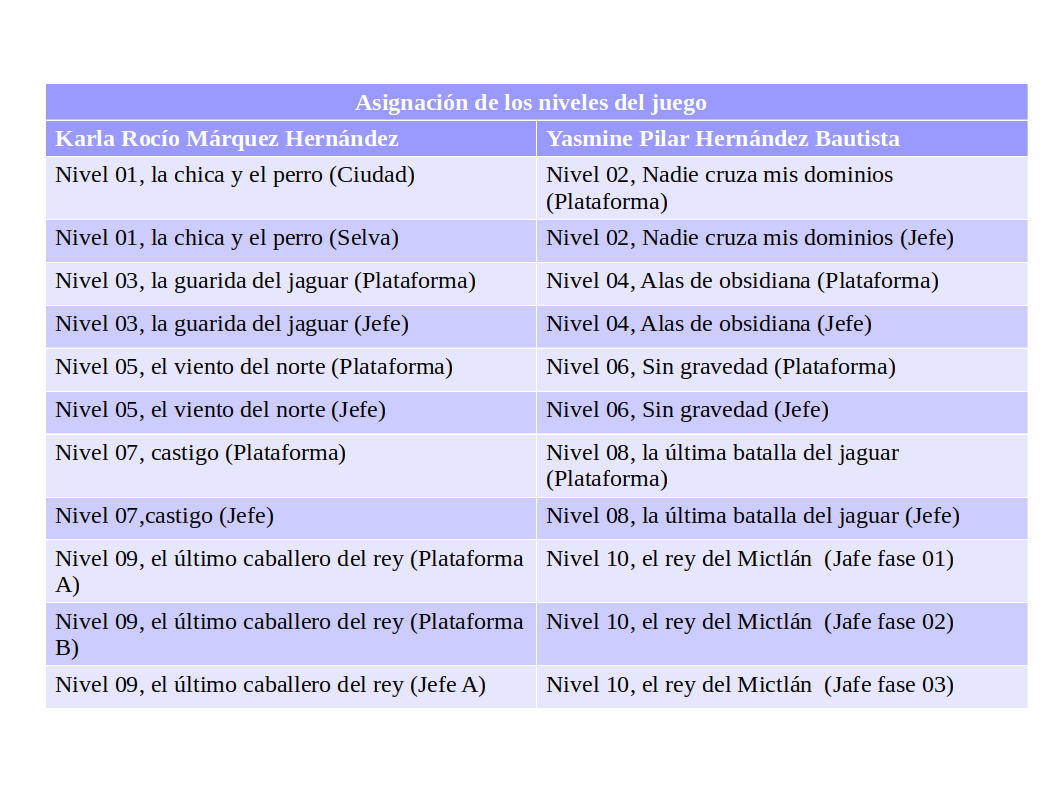
\includegraphics[width=0.8\textwidth]{02Antecedentes/Imagenes/tareasAsignacion.png}
    			\caption{Asignacion de tareas}
    			\label{fig:Tareas}
		\end{figure}


Esta división de trabajo permite que los niveles se desarrollen de manera paralela y no de manera secuencial como se había trabajado hasta este \textit{sprint}; simulando de esta forma un flujo de trabajo similar a procesamiento multihilo, en el que cada integrante del equipo es un hilo y desarrolla sus tareas de manera paralela al otro.

\subsection{Actualizando el motor de juego}
Paralelamente a la nueva asignación de tareas, fue liberada la versión 
2017.3.1f de \textit{Unity3D}. Esta versión incluye herramientas que agilizan la 
creación de niveles como el uso de: 
	\begin{itemize}
		\item \textbf{\textit{Tilemap}:} Herramienta para el mapeado de niveles. Esta 
		herramienta facilita la creación de mapas al crear una malla sobre la que 
		se arrastraran diferentes \textit{Sprites} que se hayan importado previamente 
		al tilemap (ver figura \ref{fig:TilemapPantalla}). En la sección () se 
		profundizará su funcionamiento.
		
		\begin{figure}[h]
    			\centering
    			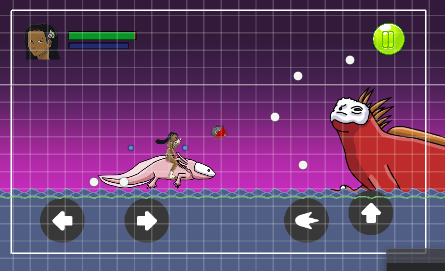
\includegraphics[width=0.6\textwidth]{02Antecedentes/Imagenes/tilemaps01.png}
    			\caption{Vista de la escena cuando se tiene un \textit{GameObject} de 
    			tipo \textit{Tilemaps} para la construcción de niveles}
    			\label{fig:TilemapPantalla}
		\end{figure}
		
		\item \textbf{\textit{Cinemachine}:} \textit{Asset} que permite controlar la 
		cámara de la escena, con este \textit{asset} se le puede indicar que objeto se 
		desea que la cámara siga y se puede asignar un área que limitara el movimiento 
		de la cámara (ver figura \ref{fig:CinemaPantalla}). \textit{Cinemachine} se 
		descarga directamente desde la tienda de \textit{assets} de \textit{Unity} y 
		fue desarrollado por los ingenieros de \textit{Unity}, lo que significa que 
		no genera conflictos o no requiere de configuraciones extras al proyecto para 
		importar. En la sección () se profundizará su funcionamiento.
			
			\begin{figure}[h]
    			\centering
    			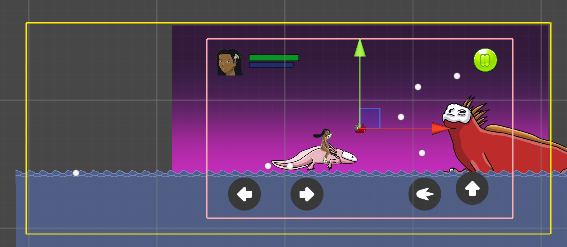
\includegraphics[width=0.6\textwidth]{02Antecedentes/Imagenes/cinemachine01.png}
    			\caption{Vista de la escena cuando se tiene un \textit{GameObject} de 
    			tipo \textit{Tilemaps} para la construcción de niveles}
    			\label{fig:CinemaPantalla}
			\end{figure}

		\item \textbf{\textit{Sprite Packer}}: Si bien no es una herramienta para 
		construcción de niveles o un \textit{asset}, esta herramienta es una de las 
		más útiles que se agregó a la nueva versión de \textit{Unity} ya que, como 
		su nombre lo indica, permite el empaquetado de \textit{sprites} (ver figura ). 
		Empaquetar 
		los \textit{sprites} es una práctica que optimiza el renderizado de objetos, 
		ya que el controlador de gráficos de \textit{Unity} realiza una sola llamada 
		por paquete cuando renderiza los objetos y con esa única llamada renderiza todos 
		los objetos de la escena que se encuentren en ese paquete; si los 
		\textit{sprites} no se encontraran dentro de un paquete el controlador de 
		gráficos de \textit{Unity} haría una llamada por cada \textit{sprite}.  
			\begin{figure}[h]
    			\centering
    			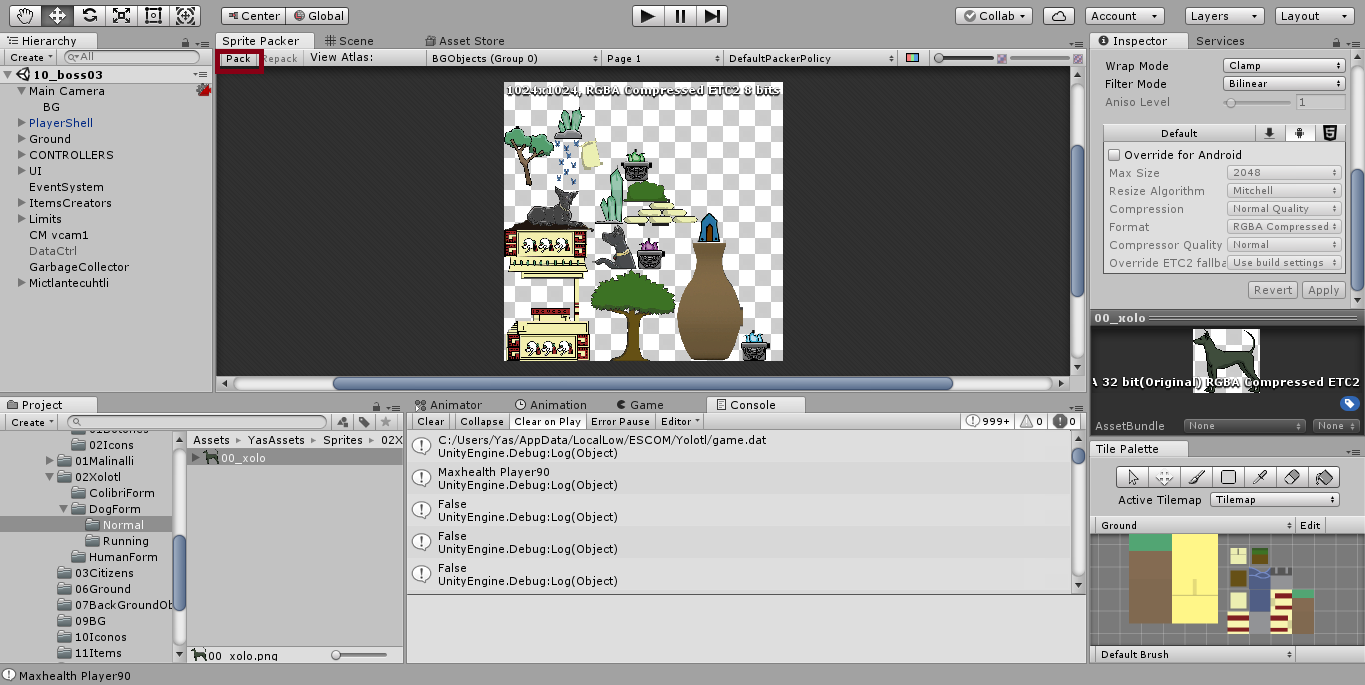
\includegraphics[width=0.6\textwidth]{02Antecedentes/Imagenes/01.png}
    			\caption{Vista de la pestaña del \textit{Sprite Packer}.}
    			\label{fig:CinemaPantalla}
			\end{figure}
	\end{itemize}
	Por el impacto que tendrían las nuevas herramientas de la versión de 
	\textit{Unity}, se propusó utilizarla en lugar de la versión 5.6.2f1. Antes 
	de actualizar la versión de \textit{Unity} se investigó si el proyecto sufriría 
	algún impacto negativo como falta de compatibilidad de componentes por la 
	diferencia de versiones. Al comprobar que existía una total compatibilidad 
	entre ambas versiones en cuanto a trasladar un proyecto de la versión 5.6.1f 
	a la versión 2017.3.1f. Se determinó que la nueva versión de \textit{Unity} 
	sería la que se emplearía para el resto del desarrollo del juego.